\documentclass[twocolumn,prl,aps,a4]{revtex4-1}
\usepackage{amsmath}
\usepackage{amssymb}
\usepackage{braket}
\usepackage{graphicx}
\usepackage[table]{xcolor}
\usepackage{verbatim}
\usepackage{float}
\usepackage{changepage}

\restylefloat{figure}

\begin{document}
\title{Deep Learning Analysis of the Oxford-IIIT Pet Dataset}
\author{Viktor Z\'{o}lyomi}

\date{\today}

\begin{abstract}
Transfer learning is used to train deep learning networks
for the purpose of classifying a database of $\approx 8000$ images.
Pre-trained networks implemented in Keras are used as base models, keeping
their weights fixed while their top layers are replaced by 2 to 5
trainable fully connected layers.
\end{abstract}

\maketitle
%

Deep neural networks (DNNs) provide a powerful tool for image classification
through the use of convolutional layers which identify features within
images. The task of training a DNN for a specific dataset is made difficult
by the computational expense of training convolutional networks of many layers,
and by the need for large datasets. A way around this is to use the method
of transfer learning \cite{DTL}. Numerous DNNs are available publicly
in the Keras library \cite{Keras}, which can be used as a starting point for
transfer learning. One simply loads the pretrained DNN, discards its top layer
which is specific to the classification task for which it was trained, then
replaces it with a small number of fully connected layers designed for
one's own image classification task at hand.

In this work, the transfer learning approach is used on a relatively modest
dataset, the Oxford-IIIT Pet Dataset \cite{PetData}. This dataset
consists of roughly 8000 total images spanning 37 different classes
of cat and dog breeds, i.e. on the order of 200 images per class. As such,
training a DNN from scratch for classifying cat and dog breeds using this dataset would
not be appropriate as sufficient accuracy requires a much bigger statistical
ensemble. Instead, three pre-trained networks available in Keras are used:
MobileNet \cite{MobileNet}, DenseNet \cite{DenseNet}, and Xception \cite{Xception},
comprising 88, 121, and 126 layers, respectively.
In each case, the top layer is replaced with 2 to 5 fully connected layers
to test the effects of increasing complexity at the top of the DNNs. Only
the newly added layers are trained, all pre-trained weights within the base
DNNs are retained. The Adam optimizer \cite{Adam} and the categorical
cross entropy loss function are used. 75\% of the images are used for training and
the rest for validation. Only the original images are used, ignoring the trimap
and bounding box information supplied with the IIIT pet dataset, in order
to gauge the effectiveness of the DNNs on the images before any manual
preprocessing.

Training was performed by a Python program making use of the Keras 2.2.4
library and the TensorFlow 1.12 \cite{TensorFlow} backend, over 20 epochs.
The source code used is hosted on GitHub \cite{GTH} along with training
history for the DNNs and png images visualizing the training metrics.

Fig. \ref{fig_acc_loss} shows the results of the training. Loss is shown
on the left, accuracy on the right. Each row corresponds to the
number of fully connected layers (2L, 3L, 4L, 5L) that were added to the
base DNNs (MobileNet, DenseNet, Xception), as labelled.

Convergence of the training loss and accuracy is achieved rapidly.
Past 10 epochs the training accuracy consistently remains greater than
95\% in all cases except for the MobileNet-based DNN with 5 extra layers,
and even in that case it is consistently above 90\%. Validation accuracy
slightly exceeds 80\% uisng MobileNet and Xception with a small improvement
using the latter. DenseNet-based DNNs underperform here with the validation
accuracy fluctuating between 65\% and 80\%, except for the case of 5 fully
connected layers at the top level, where fluctuations are even larger.

In terms of model complexity, Fig. \ref{fig_acc_loss} shows signs of
overfitting when the number of fully connected layers at the top level
increases. Validation loss rises when going from 4 to 5 layers
in both MobileNet and DenseNet, while in the Xception-based networks
the validation loss is best using just 2 fully connected layers at
top level. As mentioned, there are fluctuations present
in the validation accuracy, especially in the DenseNet-based DNNs. On
the example of the MobileNet-based DNNs training was continued for an
additional 30 epochs, i.e. a total of 50; these are stored in
the GitHub repository \cite{GTH}. The fluctuations observed in
Fig. \ref{fig_acc_loss} remain even after 50 epochs with no significant
change in the moving mean validation accuracy, suggesting that the
DNNs used here reach peak performance after 10 epochs.

It is somewhat disappointing that the training accuracy does not reach even
90\%, however, considering the small size of the training dataset this
validation accuracy is not surprising. Much higher accuracy could likely
be achieved by increasing the size of the training image dataset.

\begin{figure*}
\includegraphics[scale=0.28,angle=270]{figures/Loss_2L.eps}
\includegraphics[scale=0.28,angle=270]{figures/Accu_2L.eps}\\
\includegraphics[scale=0.28,angle=270]{figures/Loss_3L.eps}
\includegraphics[scale=0.28,angle=270]{figures/Accu_3L.eps}\\
\includegraphics[scale=0.28,angle=270]{figures/Loss_4L.eps}
\includegraphics[scale=0.28,angle=270]{figures/Accu_4L.eps}\\
\includegraphics[scale=0.28,angle=270]{figures/Loss_5L.eps}
\includegraphics[scale=0.28,angle=270]{figures/Accu_5L.eps}
\caption{
\label{fig_acc_loss} Accuracy and loss function in the 12 deep neural
networks trained in this work.
}
\end{figure*}


\begin{thebibliography}{9}%
\makeatletter
\providecommand \@ifxundefined [1]{%
 \@ifx{#1\undefined}
}%
\providecommand \@ifnum [1]{%
 \ifnum #1\expandafter \@firstoftwo
 \else \expandafter \@secondoftwo
 \fi
}%
\providecommand \@ifx [1]{%
 \ifx #1\expandafter \@firstoftwo
 \else \expandafter \@secondoftwo
 \fi
}%
\providecommand \natexlab [1]{#1}%
\providecommand \enquote  [1]{``#1''}%
\providecommand \bibnamefont  [1]{#1}%
\providecommand \bibfnamefont [1]{#1}%
\providecommand \citenamefont [1]{#1}%
\providecommand \href@noop [0]{\@secondoftwo}%
\providecommand \href [0]{\begingroup \@sanitize@url \@href}%
\providecommand \@href[1]{\@@startlink{#1}\@@href}%
\providecommand \@@href[1]{\endgroup#1\@@endlink}%
\providecommand \@sanitize@url [0]{\catcode `\\12\catcode `\$12\catcode
  `\&12\catcode `\#12\catcode `\^12\catcode `\_12\catcode `\%12\relax}%
\providecommand \@@startlink[1]{}%
\providecommand \@@endlink[0]{}%
\providecommand \url  [0]{\begingroup\@sanitize@url \@url }%
\providecommand \@url [1]{\endgroup\@href {#1}{\urlprefix }}%
\providecommand \urlprefix  [0]{URL }%
\providecommand \Eprint [0]{\href }%
\providecommand \doibase [0]{http://dx.doi.org/}%
\providecommand \selectlanguage [0]{\@gobble}%
\providecommand \bibinfo  [0]{\@secondoftwo}%
\providecommand \bibfield  [0]{\@secondoftwo}%
\providecommand \translation [1]{[#1]}%
\providecommand \BibitemOpen [0]{}%
\providecommand \bibitemStop [0]{}%
\providecommand \bibitemNoStop [0]{.\EOS\space}%
\providecommand \EOS [0]{\spacefactor3000\relax}%
\providecommand \BibitemShut  [1]{\csname bibitem#1\endcsname}%
\let\auto@bib@innerbib\@empty
%</preamble>
\bibitem [{\citenamefont {Tan}\ \emph {et~al.}()\citenamefont {Tan},
  \citenamefont {Sun}, \citenamefont {Kong}, \citenamefont {Zhang},
  \citenamefont {Yang},\ and\ \citenamefont {Liu}}]{DTL}%
  \BibitemOpen
  \bibfield  {author} {\bibinfo {author} {\bibfnamefont {C.}~\bibnamefont
  {Tan}}, \bibinfo {author} {\bibfnamefont {F.}~\bibnamefont {Sun}}, \bibinfo
  {author} {\bibfnamefont {T.}~\bibnamefont {Kong}}, \bibinfo {author}
  {\bibfnamefont {W.}~\bibnamefont {Zhang}}, \bibinfo {author} {\bibfnamefont
  {C.}~\bibnamefont {Yang}}, \ and\ \bibinfo {author} {\bibfnamefont
  {C.}~\bibnamefont {Liu}},\ }\href@noop {} {\enquote {\bibinfo {title} {A
  survey on deep transfer learning},}\ }\bibinfo {note}
  {arXiv:1808.01974}\BibitemShut {NoStop}%
\bibitem [{Ker()}]{Keras}%
  \BibitemOpen
  \href@noop {} {}\bibinfo {note} {https://keras.io}\BibitemShut {NoStop}%
\bibitem [{\citenamefont {Parkhi}\ \emph {et~al.}(2012)\citenamefont {Parkhi},
  \citenamefont {Vedaldi}, \citenamefont {Zisserman},\ and\ \citenamefont
  {Jawahar}}]{PetData}%
  \BibitemOpen
  \bibfield  {author} {\bibinfo {author} {\bibfnamefont {O.~M.}\ \bibnamefont
  {Parkhi}}, \bibinfo {author} {\bibfnamefont {A.}~\bibnamefont {Vedaldi}},
  \bibinfo {author} {\bibfnamefont {A.}~\bibnamefont {Zisserman}}, \ and\
  \bibinfo {author} {\bibfnamefont {C.~V.}\ \bibnamefont {Jawahar}},\ }in\
  \href@noop {} {\emph {\bibinfo {booktitle} {IEEE Conference on Computer
  Vision and Pattern Recognition}}}\ (\bibinfo {year} {2012})\BibitemShut
  {NoStop}%
\bibitem [{\citenamefont {Howard}\ \emph {et~al.}()\citenamefont {Howard},
  \citenamefont {Zhu}, \citenamefont {Chen}, \citenamefont {Kalenichenko},
  \citenamefont {Wang}, \citenamefont {Weyand}, \citenamefont {Andreetto},\
  and\ \citenamefont {Adam}}]{MobileNet}%
  \BibitemOpen
  \bibfield  {author} {\bibinfo {author} {\bibfnamefont {A.~G.}\ \bibnamefont
  {Howard}}, \bibinfo {author} {\bibfnamefont {M.}~\bibnamefont {Zhu}},
  \bibinfo {author} {\bibfnamefont {B.}~\bibnamefont {Chen}}, \bibinfo {author}
  {\bibfnamefont {D.}~\bibnamefont {Kalenichenko}}, \bibinfo {author}
  {\bibfnamefont {W.}~\bibnamefont {Wang}}, \bibinfo {author} {\bibfnamefont
  {T.}~\bibnamefont {Weyand}}, \bibinfo {author} {\bibfnamefont
  {M.}~\bibnamefont {Andreetto}}, \ and\ \bibinfo {author} {\bibfnamefont
  {H.}~\bibnamefont {Adam}},\ }\href@noop {} {\enquote {\bibinfo {title}
  {Mobilenets: Efficient convolutional neural networks for mobile vision
  applications},}\ }\bibinfo {note} {arXiv:1704.04861}\BibitemShut {NoStop}%
\bibitem [{\citenamefont {Huang}\ \emph {et~al.}()\citenamefont {Huang},
  \citenamefont {Liu},\ and\ \citenamefont {Weinberger}}]{DenseNet}%
  \BibitemOpen
  \bibfield  {author} {\bibinfo {author} {\bibfnamefont {G.}~\bibnamefont
  {Huang}}, \bibinfo {author} {\bibfnamefont {Z.}~\bibnamefont {Liu}}, \ and\
  \bibinfo {author} {\bibfnamefont {K.~Q.}\ \bibnamefont {Weinberger}},\
  }\href@noop {} {\enquote {\bibinfo {title} {Densely connected convolutional
  networks},}\ }\bibinfo {note} {ArXiv:1608.06993}\BibitemShut {NoStop}%
\bibitem [{\citenamefont {Chollet}()}]{Xception}%
  \BibitemOpen
  \bibfield  {author} {\bibinfo {author} {\bibfnamefont {F.}~\bibnamefont
  {Chollet}},\ }\href@noop {} {\enquote {\bibinfo {title} {Xception: Deep
  learning with depthwise separable convolutions},}\ }\bibinfo {note}
  {arXiv:1610.02357}\BibitemShut {NoStop}%
\bibitem [{\citenamefont {Kingma}\ and\ \citenamefont {Ba}()}]{Adam}%
  \BibitemOpen
  \bibfield  {author} {\bibinfo {author} {\bibfnamefont {D.~P.}\ \bibnamefont
  {Kingma}}\ and\ \bibinfo {author} {\bibfnamefont {J.~L.}\ \bibnamefont
  {Ba}},\ }\href@noop {} {\enquote {\bibinfo {title} {Adam: A method for
  stochastic optimization},}\ }\bibinfo {note} {arXiv:1412.6980}\BibitemShut
  {NoStop}%
\bibitem [{Ten()}]{TensorFlow}%
  \BibitemOpen
  \href@noop {} {}\bibinfo {note} {https://www.tensorflow.org}\BibitemShut
  {NoStop}%
\bibitem [{GTH()}]{GTH}%
  \BibitemOpen
  \href@noop {} {}\bibinfo {note} {https://github.com/zachary469/TL-DNN}
  \BibitemShut {NoStop}%
\end{thebibliography}%
\end{document}
